\documentclass[11pt]{article}
\usepackage{geometry}
\usepackage{graphicx}
\usepackage{enumitem}
\usepackage{float}
\usepackage{amsmath}
\usepackage{multicol}
\usepackage{cancel}

\geometry{a4paper, top=0.5in, bottom=0.5in, right=0.75in, left=0.75in}

\title{Lecture 2}
\author{}
\date{}

\begin{document}

\maketitle

\section{Dilute Absorbing Medium}
\begin{itemize}
    \item In order to obtain light-matter interaction for transparent media (such as fiber), we can dope this material with absorbing material (such as Erbium).
    \item $\chi = \chi_{host} + \chi_{transition}$
    \item We can ignore $\chi_{host}''$ since we are operating at a frequency away from its resonance frequency. 
\end{itemize}
\begin{align*}
    \epsilon_r &= 1 + \chi_{host} + \chi_{transition} \\
    &= \epsilon_{r_{\text{host}}} \left( 1 + \frac{\chi_{transition}}{\epsilon_{r_{\text{host}}}} \right) \\
\end{align*}
Square root to get the refractive index and $n_b$ is the refractive index of the host material:
\begin{align*}
    n_{eff} = n_b \left( 1 + \frac{\chi_{transition}}{n_b^2}\right)^{1/2} \\
\end{align*}
Assume $\chi_{transition} << n_b^2$ so that we apply Taylor expansion:
\begin{align*}
    n_{eff} &= n_b \left( 1 + \frac{\chi_{transition}}{2n_b^2}\right) \\
    &= n_b + \frac{\chi_{transition}}{2n_b} \\
    &= n_b + \frac{\chi_{transition}'}{2n_b} + j \frac{\chi_{transition}''}{2n_b} \\
\end{align*}
For a propagating wave:
\begin{align*}
    e^{-jn_{eff}k_0z} = e^{-j \left(n_b + \frac{\chi_{transition}'}{2n_b} \right)k_0z} e^{\frac{\chi_{transition}''}{2n_b}k_0z} \\
\end{align*}
Remarks:
\begin{itemize}
    \item The first term represents the phase change and the second term represents the amplitude change.
    \item $e^{\frac{k_0 \chi''z}{2n_b}} = e^{-\frac{\alpha}{2}z}$ (amplitude change)
    \item The field's amplitude decays by $\frac{\alpha}{2}$, and the power decays by $\alpha$.
\end{itemize}
Using the derived expression for $\chi''$:
\begin{align*}
    \alpha = -\frac{k_0\chi''}{n_b} = \frac{N_a q^2}{m \eta \omega \epsilon_0 n_b} \frac{k_0}{1+ \left( \frac{2(\omega - \omega_0)}{\eta} \right)^2}
\end{align*}
Multiply by $\frac{\eta^2}{\eta^2}$:
\begin{align*}
    -\frac{k_0\chi''}{n_b} &= \frac{N_a q^2}{m \eta \omega \epsilon_0 n_b} \frac{k_0 \eta^2}{\eta^2 + 4(\omega - \omega_0)^2}
\end{align*}
From $\omega = 2 \pi \nu$ and $k_0 = \frac{\omega}{c_0}$:
\begin{align*}
    \alpha &= \frac{N_a q^2}{m \eta \cancel{\omega} \epsilon_0 n_b} \frac{\cancel{\omega}}{c_0} \frac{\eta^2}{\eta^2 + 4(2 \pi (\nu - \nu_0))^2} \\
    &= \frac{N_a q^2}{m \eta \epsilon_0 n_b c_0} \frac{\eta^2}{\eta^2 + 4 (4 \pi^2)(\nu - \nu_0)^2}
\end{align*}
$4(4 \pi^2) = (4 \pi)^2$, so:
\begin{align*}
    \alpha &= \frac{N_a q^2}{m \eta \epsilon_0 n_b c_0} \frac{\left( \frac{\eta}{4 \pi} \right) ^2}{\left( \frac{\eta}{4 \pi} \right) ^2 + (\nu - \nu_0)^2} \\
    &= \frac{N_a q^2}{m \cancel{\eta} \epsilon_0 n_b c_0} \frac{\eta^{\cancel{2}}}{4(2 \pi)(2 \pi)} \frac{1}{\left( \frac{\eta}{4 \pi} \right) ^2 + (\nu - \nu_0)^2} \\
    &= \frac{N_a q^2}{m \epsilon_0 n_b c_0} \frac{\frac{1}{2 \pi} \frac{\eta}{2 \pi}}{4} \frac{1}{\left( \frac{\eta}{4 \pi} \right) ^2 + (\nu - \nu_0)^2}
\end{align*}
Let $\Delta \nu = \frac{1}{2 \pi \tau}$, so $\eta = \frac{1}{\tau} = 2 \pi \Delta \nu$, so $\Delta \nu = \frac{\eta}{2 \pi}$:
\begin{align*}
    \alpha = \frac{N_a q^2}{4m \epsilon_0 n_b c_0} \frac{\frac{\Delta \nu}{2 \pi}}{(\frac{\Delta \nu}{2})^2 + (\nu - \nu_0)^2}
\end{align*} 
Given that $\tau_r = \frac{6 \pi \epsilon_0 m c_0^3}{q^2 \omega_0^2 n_b}$, multiply by $\frac{\tau_r}{\tau_r}$:
\begin{align*}
    \alpha &= \frac{1}{\tau_r} \frac{N_a \cancel{q^2}}{4 \cancel{m} \cancel{\epsilon_0} n_b \cancel{c_0}} \frac{6 \pi \cancel{\epsilon_0} \cancel{m} c_0^{2}}{\cancel{q^2} \omega_0^2 n_b} \frac{\frac{\Delta \nu}{2 \pi}}{(\frac{\Delta \nu}{2})^2 + (\nu - \nu_0)^2} \\
    &= \frac{3 \pi N_a}{2 \tau_r} \left( \frac{c_0}{2 \pi \nu_0 n_b} \right)^2 \frac{\frac{\Delta \nu}{2 \pi}}{(\frac{\Delta \nu}{2})^2 + (\nu - \nu_0)^2}
\end{align*}
Using $c = \nu \lambda$:
\begin{align*}
    \alpha &= \frac{3 \pi N_a}{2 (4 \pi^2) \tau_r} \lambda^2 \frac{\frac{\Delta \nu}{2 \pi}}{(\frac{\Delta \nu}{2})^2 + (\nu - \nu_0)^2} \\
    &= \frac{3 N_a}{8 \pi \tau_r} \lambda^2 \frac{\frac{\Delta \nu}{2 \pi}}{(\frac{\Delta \nu}{2})^2 + (\nu - \nu_0)^2}
\end{align*}
Notes:
\begin{itemize}
    \item $\lambda$ is the wavelength inside the material ($\lambda = \frac{\lambda_0}{n}$)
    \item $f_1(\nu) = \frac{3 N_a}{8 \pi \tau_r} \lambda^2$ and $f_2(\nu) = \frac{\frac{\Delta \nu}{2 \pi}}{(\frac{\Delta \nu}{2})^2 + (\nu - \nu_0)^2}$
    \item From this derivation:
        \begin{align*}
            \nu &= \frac{c}{\lambda} \\
            \frac{d \nu}{d \lambda} &= -\frac{c}{\lambda^2} \\
            \Delta \nu &= -\frac{c}{\lambda^2} \Delta \lambda \\
            \Delta \lambda &= -\frac{\lambda^2}{c} \Delta \nu
        \end{align*}
        Since $\lambda^2$ is in $10^{-12}$ range, and $\frac{1}{c}$ is in $10^{-8}$ range, so any change in frequency ($\Delta \nu$) will be multiplied by $10^{-20}$. We can conclude that $f_1(\nu)$ is a very slowly varying function of $\nu$ and can be considered as a constant.
    \item $f_2(\nu)$ has a Lorentzian shape and is called the line shape function
    \begin{align*}
        g_{\nu_0}(\nu) = \frac{\frac{\Delta \nu}{2 \pi}}{(\frac{\Delta \nu}{2})^2 + (\nu - \nu_0)^2}
    \end{align*}
        \begin{itemize}
            \item Maximum at $\nu = \nu_0$
                \begin{align*}
                    g_{\nu_0}(\nu_0) = \frac{\frac{\Delta \nu}{2 \pi}}{(\frac{\Delta \nu}{2})^2 + (\nu_0 - \nu_0)^2} = \frac{\frac{\Delta \nu}{2 \pi}}{(\frac{\Delta \nu}{2})^2} = \frac{2}{\pi \Delta \nu}
                \end{align*}
            \item FWHM is at $\nu = \nu_0 \pm \frac{\Delta \nu}{2}$
                \begin{align*}
                    g_{\nu_0}(\nu_0 \pm \frac{\Delta \nu}{2}) = \frac{\frac{\Delta \nu}{2 \pi}}{(\frac{\Delta \nu}{2})^2 + (\frac{\Delta \nu}{2})^2} = \frac{\frac{\Delta \nu}{2 \pi}}{2(\frac{\Delta \nu}{2})^2} = \frac{1}{\pi \Delta \nu}
                \end{align*}
        \end{itemize}
    \item Note that the line shape function is normalized:
        \begin{align*}
            \int_{-\infty}^{\infty} g_{\nu_0}(\nu) d\nu = 1
        \end{align*}
    \item Classically, $\alpha$ is always positive meaning that only attenuation is possible (no amplification).
\end{itemize}

\section{Absorption Cross Section}
\begin{align*}
    \alpha = \frac{3 N_a \lambda^2}{8 \pi \tau_r} g_{\nu_0}(\nu) = N_a \sigma(\nu_0) 
\end{align*}
where $\sigma(\nu_0) = \frac{3 \lambda^2}{8 \pi \tau_r} g_{\nu_0}(\nu)$ is the absorption cross section. 
\begin{align*}
    I &= I_0 e^{-\alpha z} = I_0 e^{-N_a \sigma z} \\
    \frac{dI}{dz} &= -N_a \sigma I_0 e^{-N_a \sigma z} = -N_a \sigma I \\
    \frac{-dI}{I} &= N_a \sigma dz = \frac{\text{\# atoms}}{A \cancel{dz}} \sigma \cancel{dz} \\
\end{align*}
where:
\begin{itemize}
    \item $\frac{-dI}{I}$ is the fractional change in intensity (decrease in intensity)
    \item $N_a$ is the atomic density (number of atoms per unit volume)
    \item $\sigma$ is the absorption cross section (represents an opaque area in the material)
\end{itemize}

\section{Broadening of Spectral Lines}
\subsection{Homogeneous Broadening}
All atoms have the same resonance frequency and Lorentzian shape. The total summation of all the Lorentzian functions is a Lorentzian function.
\begin{itemize}
    \item Natural / Lifetime Broadening
    \item Collision Broadening
\end{itemize}
\begin{center}
    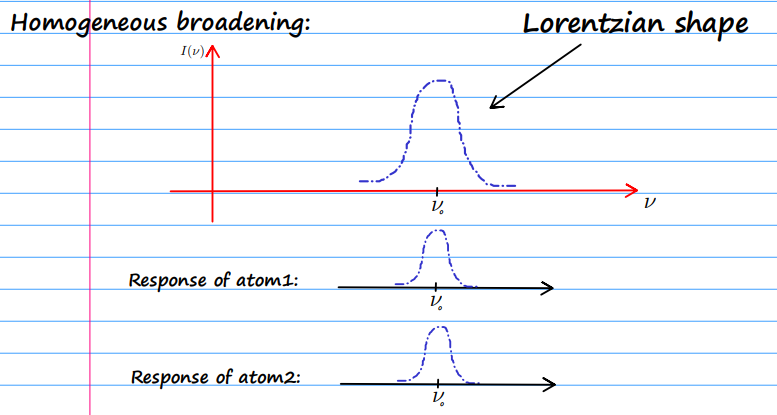
\includegraphics[scale=0.6]{1.png}
\end{center}

\subsection{Inhomogeneous Broadening}
Each group of atoms has a different resonance frequency and line shape function. The total summation of all the Lorentzian functions is a Gaussian function.
\begin{itemize}
    \item Doppler Broadening
\end{itemize}
\begin{center}
    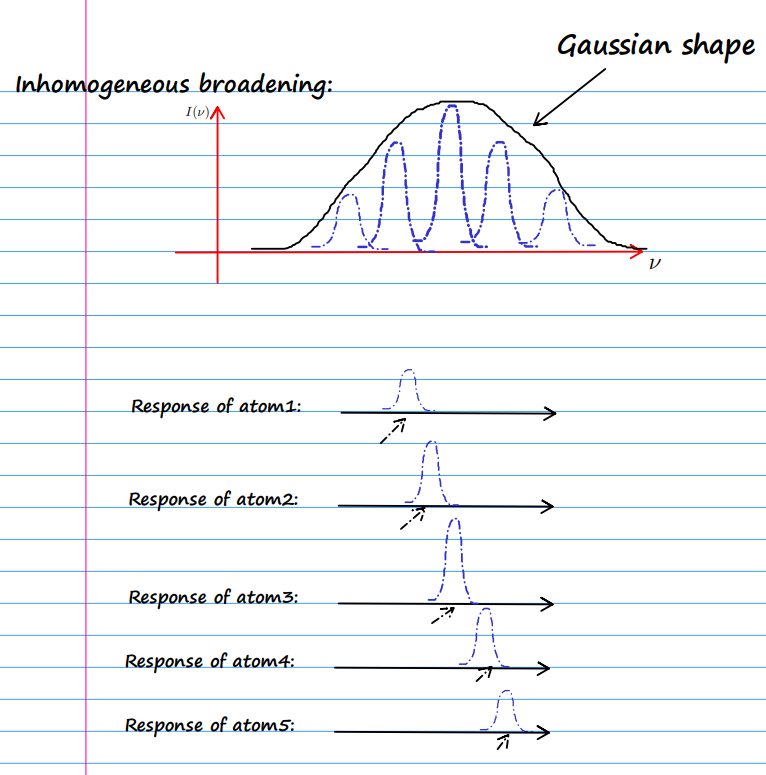
\includegraphics[scale=0.6]{2.png}
\end{center}

\subsubsection{Doppler Broadening}
\begin{itemize}
    \item Due to the randomness of the atoms' velocities and directions of motion, each atom will experience the light at a different frequency. 
    \item This usually happens in gases where the atoms are free to move.
    \item Examples:
        \begin{itemize}
            \item Atom is moving towards the light
                \begin{align*}
                    \nu_{atom} = \nu_{source} \left( 1 + \frac{v}{c} \right)
                \end{align*}
            \item Atom is moving away from the light
                \begin{align*}
                    \nu_{atom} = \nu_{source} \left( 1 - \frac{v}{c} \right)
                \end{align*}
            \item Atom is moving in the speed of light
                \begin{align*}
                    \nu_{atom} = \nu_{source} \left( 1 - \frac{c}{c} \right) = 0
                \end{align*}
        \end{itemize}
\end{itemize}
We want to get the source frequency ($\nu_{source} = \nu_0'$) equivalent to the atom's resonance frequency ($\nu_{atom} = \nu_0$)
\begin{align*}
    \nu_0' = \frac{\nu_0}{\left( 1 - \frac{v}{c} \right)} \approx \nu_0 \left( 1 + \frac{v}{c} \right)
\end{align*}
Modify the line shape function:
\begin{align*}
    g_{\nu_0}(\nu) &= \frac{\frac{\Delta \nu}{2 \pi}}{(\frac{\Delta \nu}{2})^2 + (\nu - \nu_0')^2} \\
    &= \frac{\frac{\Delta \nu}{2 \pi}}{(\frac{\Delta \nu}{2})^2 + (\nu - \nu_0(1 + \frac{v}{c}))^2} \\
\end{align*}
There is multiple line shape functions depending on the velocities of the atoms, so we need to average over all the velocities:
\begin{align*}
    \overline{g_{\nu_0}} &= \int_{-\infty}^{\infty} g(\nu) f(v) dv
\end{align*}
where $f(v)$ is the probability density function (PDF) of the velocities. From statistical thermodynamics, the PDF of the velocities is a Gaussian function with zero mean (no external force applied) and variance $\sigma_v^2$:
\begin{align*}
    f(v) = \frac{1}{\sqrt{2 \pi} \sigma_v} e^{-\frac{v^2}{2 \sigma_v^2}}
\end{align*}
The variance is given by:
\begin{align*}
    \sigma_v^2 &= E[v^2] - \cancel{E[v]^2} = \frac{k_BT}{m}
\end{align*}
So:
\begin{align*}
    \overline{g_{\nu_0}(\nu)} = \int_{-\infty}^{\infty} \frac{\frac{\Delta \nu}{2 \pi}}{(\frac{\Delta \nu}{2})^2 + (\nu - \nu_0(1 + \frac{v}{c}))^2} \frac{1}{\sqrt{2 \pi} \sigma_v} e^{-\frac{v^2}{2 \sigma_v^2}} dv
\end{align*}
This is a very difficult integral to solve, so we can solve at 2 limits:
\begin{itemize}
    \item \textbf{$\sigma_v \rightarrow 0$:} This means that the variance in atoms' velocities is very small, so the shift in resonance frequency ($\nu_0$) is very small, so the overall line shape function is a Lorentzian function (Homogeneous Broadening).
        \begin{center}
            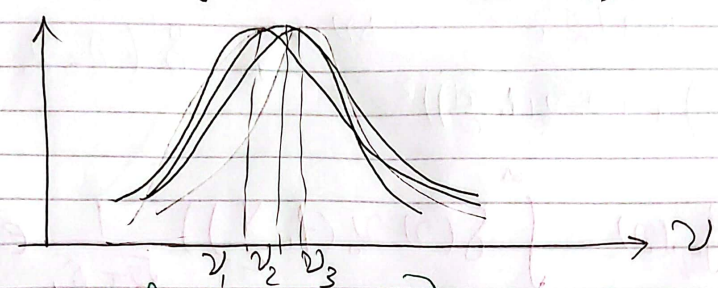
\includegraphics[scale=0.6]{3.png}
        \end{center}
    \item \textbf{$\Delta \nu \rightarrow 0$:} This means that the line width is very small that for each velocity the line shape function can be considered as a delta function (Inhomogeneous Broadening).
        \begin{center}
            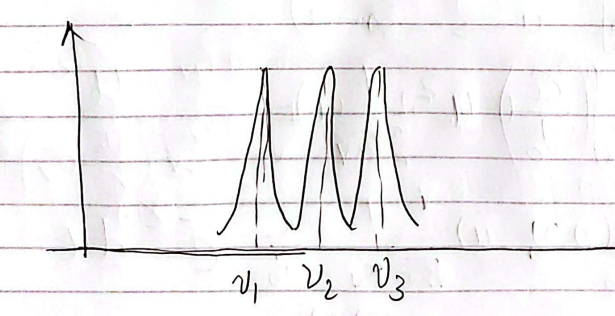
\includegraphics[scale=0.6]{4.png}
        \end{center}
\end{itemize}
For $\Delta \nu \rightarrow 0$:
\begin{align*}
    \frac{\frac{\Delta \nu}{2 \pi}}{(\frac{\Delta \nu}{2})^2 + (\nu - \nu_0(1 + \frac{v}{c}))^2}
    &= \delta \left( \nu - \nu_0 \left(1 + \frac{v}{c} \right) \right)
\end{align*}
So:
\begin{align*}
    \overline{g_{\nu_0}(\nu)} = \int_{-\infty}^{\infty} \delta \left( \nu - \nu_0 \left(1 + \frac{v}{c} \right) \right) \frac{1}{\sqrt{2 \pi} \sigma_v} e^{-\frac{v^2}{2 \sigma_v^2}} dv
\end{align*}
To utilitize $\int_{-\infty}^{\infty} \delta(x-x_0) f(x) dx = f(x_0)$, let:
\begin{align*}
    &u = \nu_0 \frac{v}{c} \Rightarrow v = \frac{c}{\nu_0} u \Rightarrow dv = \frac{c}{\nu_0} du \\
    &v \rightarrow -\infty \Rightarrow u \rightarrow -\infty \\
    &v \rightarrow \infty \Rightarrow u \rightarrow \infty
\end{align*}
Delta function will be:
\begin{align*}
    \delta \left( \nu - \nu_0 \left(1 + \frac{v}{c} \right) \right) = \delta (\nu - \nu_0 - u)
\end{align*}
The Gaussian function will be:
\begin{align*}
    \frac{1}{\sqrt{2 \pi} \sigma_v} e^{-\frac{v^2}{2 \sigma_v^2}} dv = \frac{1}{\sqrt{2 \pi} \sigma_v} e^{-\left( \frac{c}{\nu_0 \sigma_v} \right)^2 \frac{u^2}{2}} \frac{c}{\nu_0} du
\end{align*}
Let $\sigma_d = \frac{\nu_0 \sigma_v}{c}$, where $\sigma_d$ is the standard deviation of the Doppler Broadening (depends on temperature):
\begin{align*}
    \overline{g_{\nu_0}(\nu)} &= \int_{-\infty}^{\infty} \delta (\nu - \nu_0 - u) \frac{1}{\sqrt{2 \pi} \sigma_d} e^{\frac{u^2}{2 \sigma_d^2}} du \\
\end{align*}
Since the delta function is even, we can multiply by -1 inside the bracket:
\begin{align*}
    \overline{g_{\nu_0}(\nu)} &= \int_{-\infty}^{\infty} \delta (u - (\nu - \nu_0)) \frac{1}{\sqrt{2 \pi} \sigma_d} e^{-\frac{u^2}{2 \sigma_d ^2}} du \\
    &= \frac{1}{\sqrt{2 \pi} \sigma_d} e^{-\frac{(\nu - \nu_0)^2}{2 \sigma_d^2}}
\end{align*}
The final value is the Gaussian envelope of the Doppler Broadening.

\end{document}